% Visão geral do experimento (figura do paper). Compilar: pdflatex overview.tex -> overview.pdf
\documentclass[tikz,border=2pt]{standalone}
\usepackage[T1]{fontenc}
\usepackage[utf8]{inputenc}
\usepackage{libertine}
\usetikzlibrary{positioning,arrows.meta,calc}
\definecolor{tinta}{HTML}{3B2A20}
\definecolor{ga}{HTML}{6B4430}
\definecolor{gb}{HTML}{8A6C55}
\definecolor{gc}{HTML}{5E6849}
\definecolor{fundo}{HTML}{F3EEE8}
\begin{document}
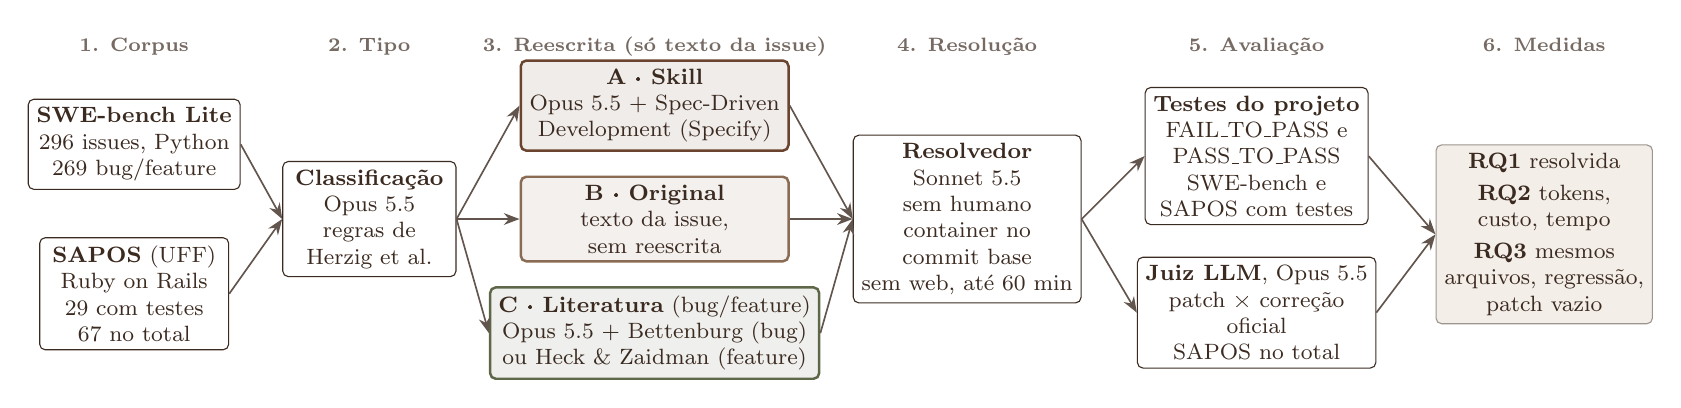
\begin{tikzpicture}[
  font=\footnotesize, text=tinta, node distance=4mm and 6mm,
  caixa/.style={draw=tinta, rounded corners=2pt, align=center, inner sep=3pt, minimum width=#1},
  caixa/.default=24mm,
  grupo/.style={draw=#1, line width=0.9pt, fill=#1!10, rounded corners=2pt, align=center, inner sep=3pt, minimum width=34mm},
  etapa/.style={font=\scriptsize\bfseries, text=tinta!70, anchor=base},
  seta/.style={-{Stealth[length=2mm]}, draw=tinta!80, line width=0.6pt}]

% 1. Corpus
\node[caixa] (swe) {\textbf{SWE-bench Lite}\\296 issues, Python\\269 bug/feature};
\node[caixa, below=6mm of swe] (sapos) {\textbf{SAPOS} (UFF)\\Ruby on Rails\\29 com testes\\67 no total};
\coordinate (meio) at ($(swe.east)!0.5!(sapos.east)$);

% 2. Tipo
\node[caixa=22mm, right=6mm of meio] (cls) {\textbf{Classificação}\\Opus 5.5\\regras de\\Herzig et al.};

% 3. Gerador
\node[grupo=gb, right=8mm of cls] (b) {\textbf{B · Original}\\texto da issue,\\sem reescrita};
\node[grupo=ga, above=3mm of b] (a) {\textbf{A · Skill}\\Opus 5.5 + Spec-Driven\\Development (Specify)};
\node[grupo=gc, below=3mm of b] (c) {\textbf{C · Literatura} (bug/feature)\\Opus 5.5 + Bettenburg (bug)\\ou Heck \& Zaidman (feature)};

% 4. Resolução
\node[caixa=24mm, right=8mm of b] (res) {\textbf{Resolvedor}\\Sonnet 5.5\\sem humano\\container no\\commit base\\sem web, até 60 min};

% 5. Avaliação
\node[caixa=27mm, right=8mm of res, yshift=8mm] (testes) {\textbf{Testes do projeto}\\FAIL\_TO\_PASS e\\PASS\_TO\_PASS\\SWE-bench e\\SAPOS com testes};
\node[caixa=27mm, below=4mm of testes] (juiz) {\textbf{Juiz LLM}, Opus 5.5\\patch × correção\\oficial\\SAPOS no total};

% 6. Medidas
\node[caixa=26mm, fill=fundo, draw=tinta!50, right=8mm of $(testes.east)!0.5!(juiz.east)$] (rq) {\textbf{RQ1} resolvida\\[2pt]\textbf{RQ2} tokens,\\custo, tempo\\[2pt]\textbf{RQ3} mesmos\\arquivos, regressão,\\patch vazio};

% setas
\draw[seta] (swe.east) -- (cls.west);
\draw[seta] (sapos.east) -- (cls.west);
\foreach \g in {a,b,c} {
  \draw[seta] (cls.east) -- (\g.west);
  \draw[seta] (\g.east) -- (res.west);
}
\draw[seta] (res.east) -- (testes.west);
\draw[seta] (res.east) -- (juiz.west);
\draw[seta] (testes.east) -- (rq.west);
\draw[seta] (juiz.east) -- (rq.west);

% rótulos das etapas
\path (a.north) ++(0,1mm) coordinate (topo);
\node[etapa] at (swe.north |- topo) {1. Corpus};
\node[etapa] at (cls.north |- topo) {2. Tipo};
\node[etapa] at (topo) {3. Reescrita (só texto da issue)};
\node[etapa] at (res.north |- topo) {4. Resolução};
\node[etapa] at (testes.north |- topo) {5. Avaliação};
\node[etapa] at (rq.north |- topo) {6. Medidas};
\end{tikzpicture}
\end{document}
